\chapter{Grundlagen}
\label{ch:Grundlagen}

Dieses Kapitel soll eine Grundlage für jeden Leser schaffen. Es werden die grundlegenden Rahmenbedingungen beschrieben, erste Begriffe und Notationen eingeführt um das spätere Verständnis des Originalwerks zu erläutern. So wird auf den folgenden Seiten ein symmetrisches Verschlüsselungs"-schema $\Pi$ und dessen Subversion $\widetilde{\Pi}$ behandelt. Subversionen sind von $\mathscr{B}$ in das Schema eingeschleuste Komponenten, die ein Key Recovery ermöglichen sollen.

\begin{section}{Die ideale Welt}
\label{sec:ideale_welt}

Als Basis für alle Erläuterungen dient ein Model der idealen Welt (siehe Abbildung \ref{fig:ideale_welt}). In einer idealen Welt möchte Alice eine verschlüsselte Nachricht $M$ an Bob schicken. Alice und Bob sind normale Nutzer, die im Besitz eines symmetrischen Schlüssels $\mathcal{K}$ sind. Für diese Übertragung wird ein symmetrisches Verschlüsselungs"-schema $\Pi = (\mathcal{E}, \mathcal{D}, \mathcal{K})$ verwendet. Das Schema $\Pi$ besteht aus einer Funktion $\mathcal{E} = (\mathcal{K}, M)$, die mit dem symmetrischen Schlüssel $\mathcal{K}$ die Nachricht $M$ verschlüsseln und eine Funktion $\mathcal{D} = (\mathcal{K}, \mathcal{C})$, die mit dem symmetrischen Schlüssel $\mathcal{K}$ einen Chiffretext $\mathcal{C}$ entschlüsselt. So ergibt sich eine erste allgemeine Definition eines symmetrischen Verschlüsselungsschemas. Big Brother $\mathscr{B}$ versucht in diesem Fall passiv die Nachricht zu entschlüsseln oder den Schlüssel $\mathcal{K}$ zu reproduzieren. Diese Art von Darstellung von Abbildung \ref{fig:ideale_welt} werde ich noch mehrfach in der Arbeit verwenden. Im oberen Teil ist immer die ideale Welt und unten sind Bestandteile des Schemas durch Subversionen ausgetauscht. In diesem Fall ist die Verschlüsselungsfunktion $\mathcal{E}$ durch die Subversion $\widetilde{\mathcal{E}}$ ausgetauscht worden. Big Brother ist in der Lage, die Nachricht mit dem Masterschlüssel $\widetilde{\mathcal{K}}$ zu reproduzieren, wobei Bob die Nachricht weiterhin entschlüsseln kann.

\begin{figure}[!ht]
	\centering
	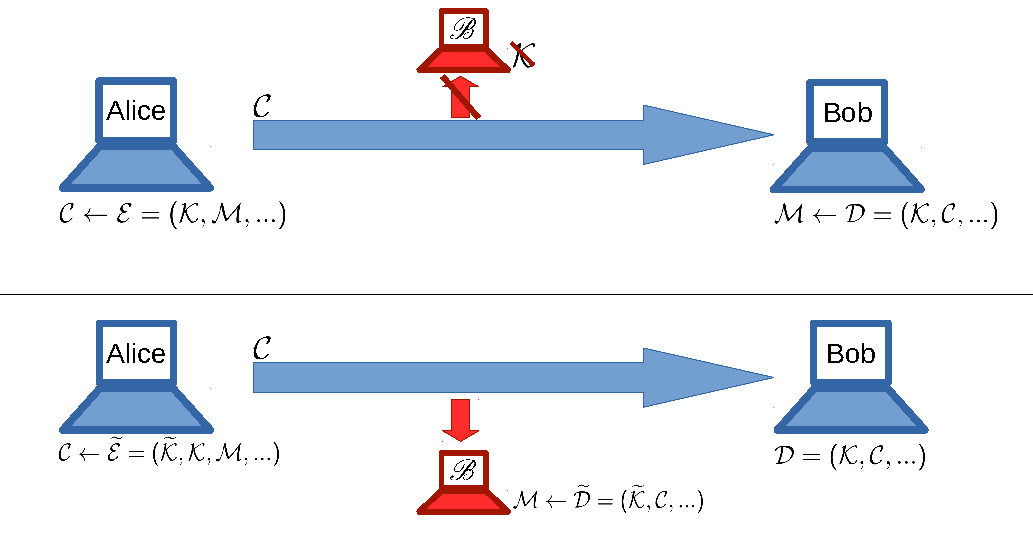
\includegraphics[width=\textwidth]{image/ideale_welt}
	\caption{Symmetrische Verschlüsselung in einer idealen Welt.}
	\label{fig:ideale_welt}
\end{figure}

\end{section}

\begin{section}{Korrektheit}
\label{sec:korrekt}

Letzteres ist essenzieller Bestandteil von Big Brothers Subversion. Jede Nachricht $M$ die von Alice verschlüsselt versendet wird muss mithilfe von $\mathcal{K}$ von Bob wieder zu $M$ entschlüsselt werden. Eben auch wenn Alice eine Subversion von $\Pi$ verwendet. Wir können sagen, dass ein Schema $\Pi = (\mathcal{K}, \mathcal{E}, \mathcal{D})$ korrekt ist, wenn der Empfänger den Chiffretext immer zu der gleichen ursprünglichen Nachricht $M$ entschlüsselt, die der Sender gesendet hat. Also wenn für alle Nachrichten gilt: $\mathcal{E}(\mathcal{K}, M_{1}) = \mathcal{C}_{1}$ und $\mathcal{D}(\mathcal{K}, \mathcal{C}_{2}) = M_{2}$, mit $\mathcal{C}_{1} = \mathcal{C}_{2}$ und $M_{1} = M_{2}$.

\end{section}

\begin{section}{Decryptability}
\label{sec:decryptability}

Eine weitere wichtige Eigenschaft beschreibt die Entschlüsselbarkeit einer Subversion $\widetilde{\Pi}$ relativ zu $\Pi$. Wenn $\widetilde{\Pi}$ ein korrektes Verschlüsselungs"-schema ist und die Funktion $\widetilde{\mathcal{E}}$ den Schlüssel $K$ und den Masterschlüssel $\widetilde{\mathcal{K}}$ verwendet, mit $K \neq \widetilde{\mathcal{K}}$, dann erfüllt $\widetilde{\Pi}$ die Eigenschaft Entschlüsselbarkeit. Allerdings nur jemand, der $\mathcal{K}$ hält, darf mit der Funktion $\mathcal{D}$ die Nachricht korrekt entschlüsseln. Wir gehen davon aus, dass $\mathscr{B}$ immer versucht diese Eigenschaft zu erreichen um nicht entdeckt zu werden.

\end{section}

\begin{section}{Detection Advantage}

Die Erfolgschancen von ASAs können an der Entdeckbarkeit gemessen werden. Eine Subversion ist von Alice oder Bob entdeckbar, wenn nicht gesagt werden kann, ob der Chiffretext $C$ von einer Subversion oder vom eigentlichen Schema $\Pi$ erzeugt wurde. Die Eigenschaft Entschlüsselbarkeit bildet hierfür die Basis. Wenn eine Entschlüsselung fehlschlägt, führt dies wahrscheinlich auch zum Entdecken der Subversion. Allerdings ist anzumerken, dass selbst wenn die Wahrscheinlichkeit Entdeckt zu werden hoch ist, beutet es nicht, dass ein Nutzer in der Lage ist eine Subversion zu entdecken.

\end{section}